\section{TỔNG QUAN VÀ THIẾT KẾ TOPOLOGY}

\subsection{Giới thiệu bài toán}
Trong kỷ nguyên kỹ thuật số hiện đại, việc xây dựng một hệ thống mạng doanh nghiệp không chỉ dừng lại ở yêu cầu về kết nối mà còn đòi hỏi khả năng bảo mật cao và tính sẵn sàng liên tục. Đồ án này tập trung vào việc thiết kế và triển khai một hệ thống mạng Campus 3 lớp tiêu chuẩn (Core - Distribution - Access) có tích hợp vùng biên DMZ (Demilitarized Zone) để đặt các dịch vụ công cộng. Bên cạnh đó, hệ thống còn được trang bị các cơ chế phòng thủ đa tầng và khả năng tự động cân bằng tải (Load Balancing) dựa trên ngưỡng băng thông định trước.

\subsection{Kịch bản giả định: Hệ thống mạng Văn phòng 2 tầng}
Để đồ án mang tính thực tiễn, hệ thống mạng được thiết kế dựa trên nhu cầu của một văn phòng doanh nghiệp quy mô trung bình (khoảng 50 nhân viên) với kịch bản như sau:
\begin{itemize}
    \item \textbf{Tầng 1 (Vùng mạng 192.168.10.0/24):} Khu vực dành cho Ban Giám đốc, phòng Kế toán và Hành chính. Đây là vùng mạng ưu tiên cao, chứa các thiết bị quan trọng như máy in mạng (IP Printer: \texttt{192.168.10.50}) và hệ thống IP Phone (\texttt{.100} - \texttt{.110}).
    \item \textbf{Tầng 2 (Vùng mạng 192.168.20.0/24):} Khu vực dành cho phòng Marketing, bộ phận Chăm sóc khách hàng và Khách vãng lai. Vùng này có tính bảo mật thấp hơn và bị hạn chế truy cập vào một số tài nguyên quản trị.
    \item \textbf{Vùng DMZ:} Chứa hệ thống Portal nội bộ và CRM phục vụ truy cập từ Internet.
\end{itemize}

\subsection{Thiết kế Topology mạng 3 lớp tích hợp HA}
Mô hình mạng được xây dựng trên môi trường ảo hóa Mininet kết hợp với FRRouting. Điểm cải tiến quan trọng nhất là tính sẵn sàng cao (High Availability):
\begin{itemize}
    \item \textbf{Vùng Access (Lớp truy cập):} Gồm Switch \texttt{acc1} và \texttt{acc2} kết nối trực tiếp đến các máy trạm của nhân viên tại hai tầng.
    \item \textbf{Vùng Distribution (Lớp phân phối):} Gồm Router \texttt{dist1} và \texttt{dist2}. Tại đây, một liên kết dự phòng (\textbf{HA Link}) đã được thiết lập nối trực tiếp giữa hai Router này.
    \item \textbf{Vùng Core (Lớp lõi):} Chịu trách nhiệm luân chuyển dữ liệu tốc độ cao lên Firewall.
    \item \textbf{Cơ chế chịu lỗi (Fault Tolerance):} Trong trường hợp đường truyền chính từ \texttt{dist1} lên \texttt{core} bị đứt, giao thức OSPF sẽ tự động định tuyến lưu lượng đi qua HA Link sang \texttt{dist2} để ra Internet, đảm bảo công việc tại văn phòng không bị gián đoạn.
\end{itemize}


\subsection{Thiết kế Sâu và Tính sẵn sàng cao (High Availability)}
Để đạt được mức độ vận hành tin cậy (Mức 3), hệ thống được tinh chỉnh với các nâng cấp sau:
\begin{itemize}
    \item \textbf{Lý do đặt thiết bị Layer 3 tại lớp Distribution:} Thay vì cấu hình Layer 3 tại Access, việc đặt Gateway tại Distribution giúp giới hạn phạm vi của Broadcast Domain xuống mức thấp nhất, giảm thiểu gánh nặng xử lý cho các switch Access rẻ tiền. Điều này giúp tối ưu hóa chi phí đầu tư thiết bị đầu cuối mà vẫn đảm bảo hiệu suất định tuyến mạnh mẽ.
    \item \textbf{Đường Link dự phòng (Redundant Link):} Hệ thống thiết lập một đường link kết nối trực tiếp giữa \texttt{dist1} và \texttt{dist2}. Đây là cơ chế HA vật lý, đảm bảo nếu một đường link chính lên Core bị đứt, OSPF sẽ tự động tìm đường đi thay thế qua router Distribution còn lại, duy trì kết nối cho người dùng.
\end{itemize}

\begin{figure}[H]
    \centering
    % [HUONG DAN]: Chạy script scripts/draw_topology.py (nếu có) hoặc dùng công cụ vẽ sơ đồ
    % để tạo ảnh topology. Đặt tên là "topology_mmtnc.png" trong thư mục image/.
    % 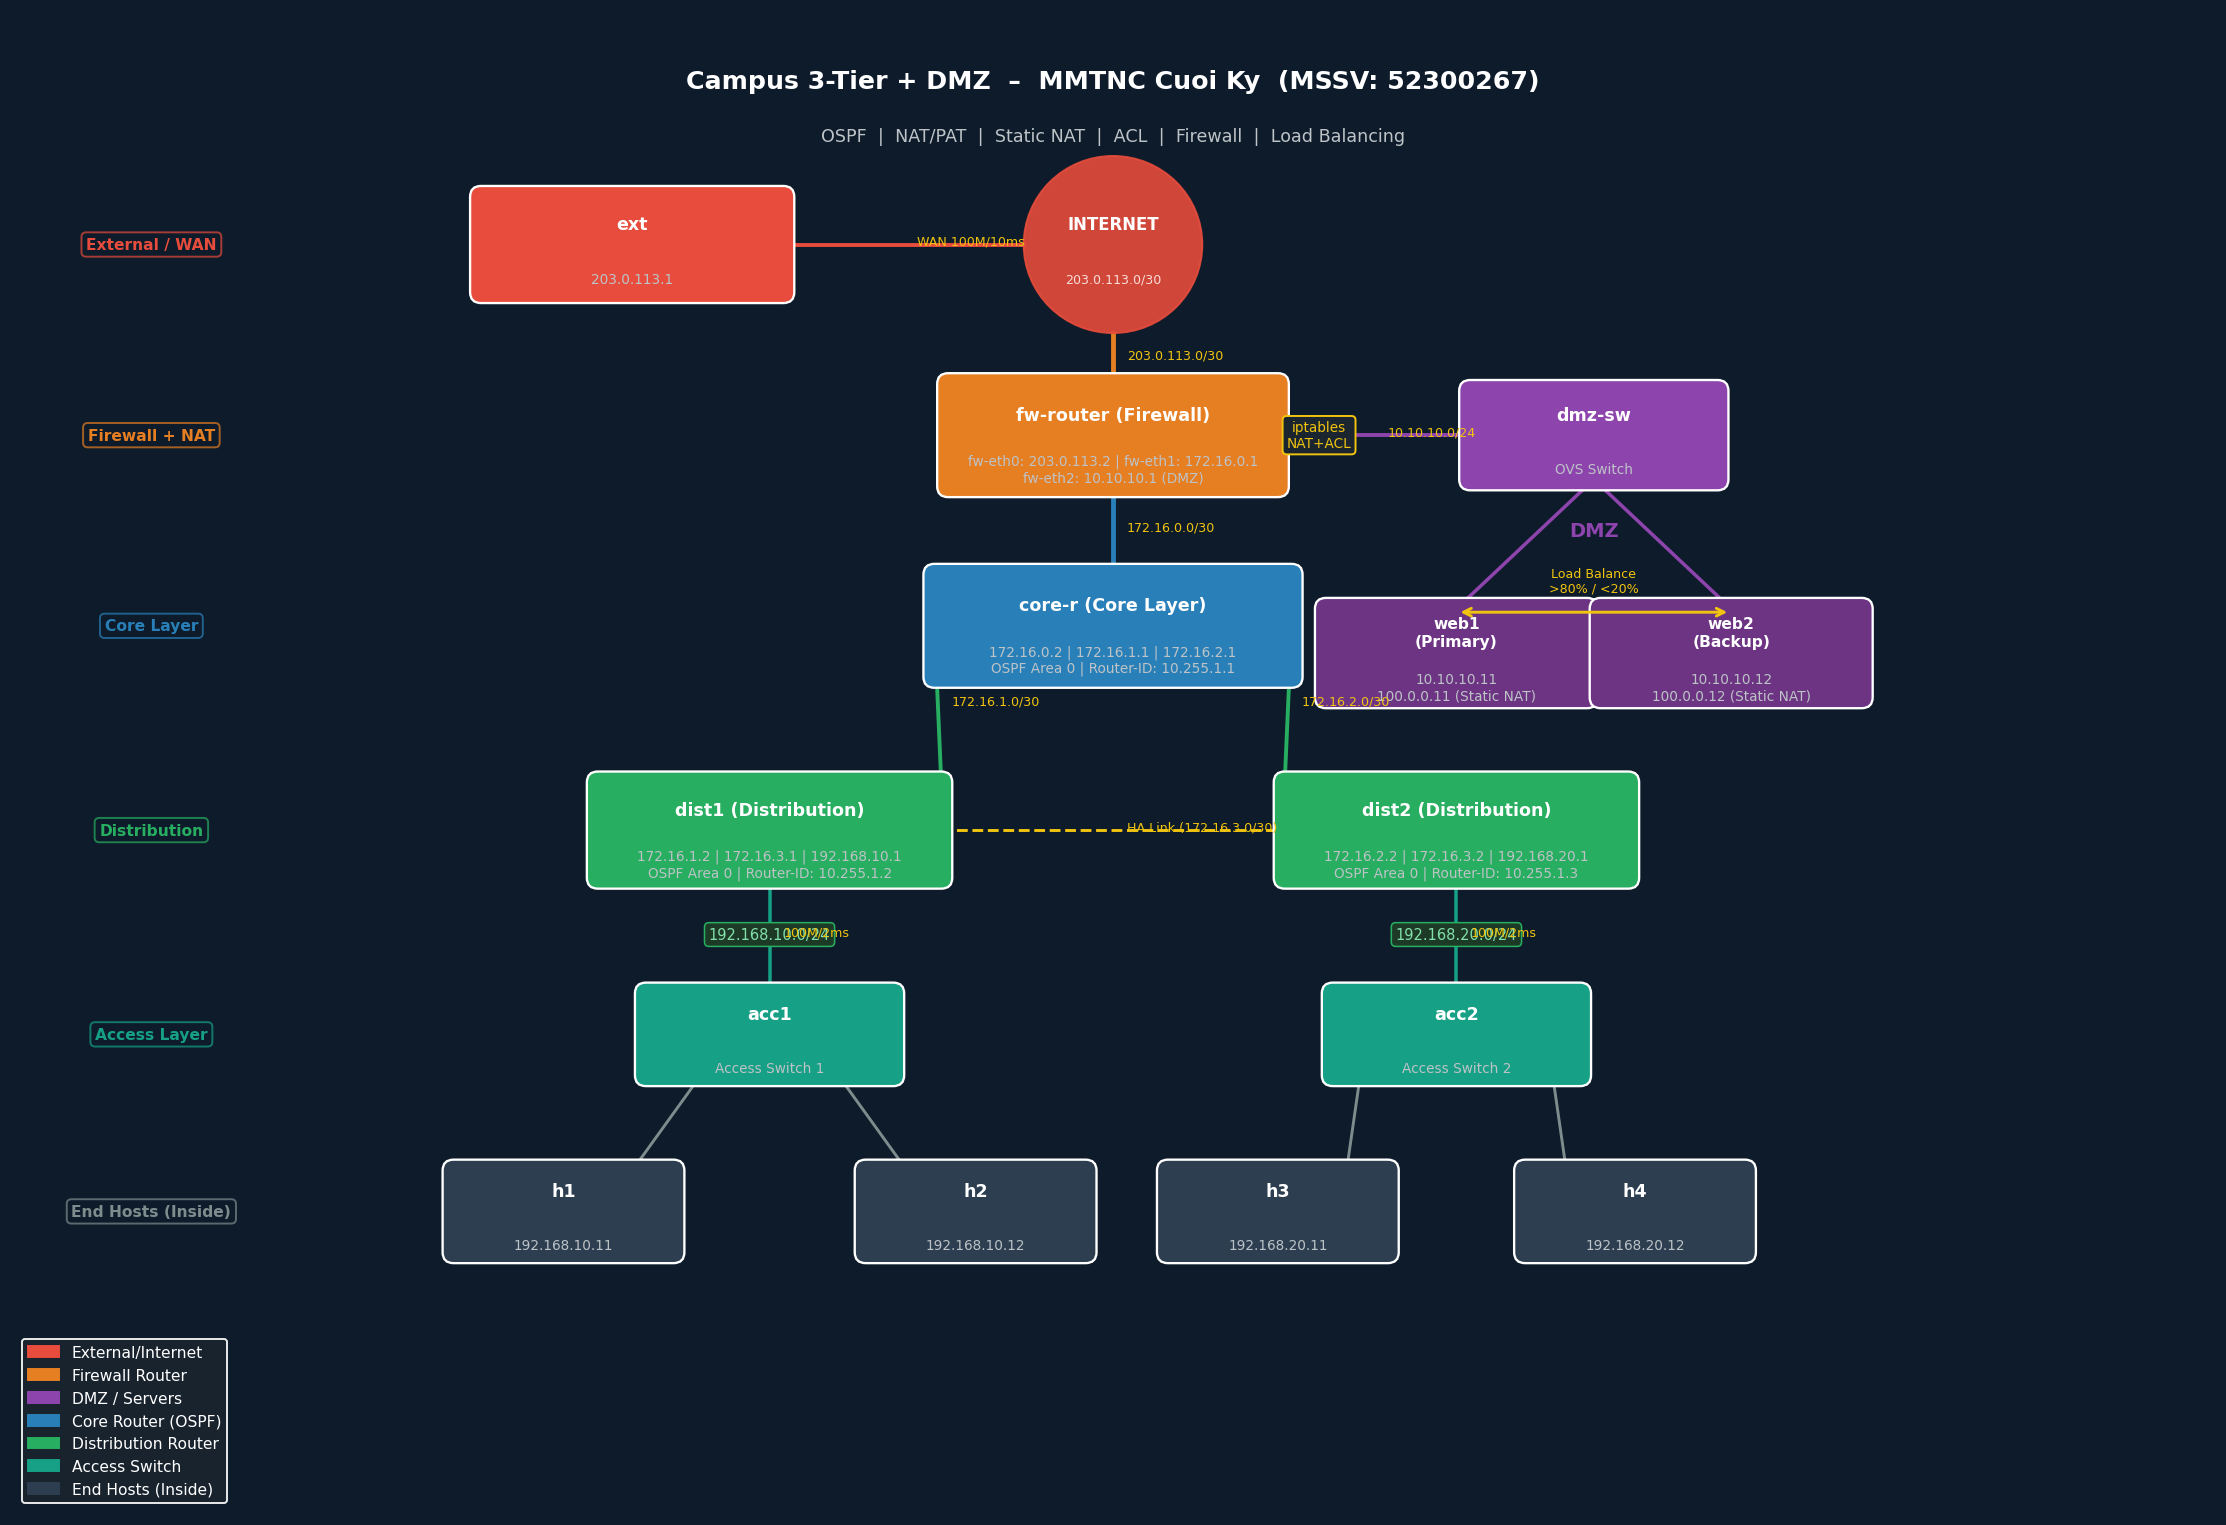
\includegraphics[width=1\textwidth]{image/topology_mmtnc.png}
    \caption{Sơ đồ thực tế hệ thống mạng Campus 3 lớp, vùng DMZ và đường HA Link}
    \label{fig:topology_actual}
\end{figure}
\textit{\textbf{Giải thích minh chứng:} Hình \ref{fig:topology_actual} thể hiện cấu trúc kết nối thực tế. Điểm nhấn quan trọng là đường nối giữa hai router Distribution, tạo thành một kiến trúc mạng có khả năng chịu lỗi (Fault-tolerant Architecture).}

\subsection{Kiểm chứng cấu hình thực tế so với thiết kế}
Để đảm bảo hệ thống vận hành đúng như bản vẽ kỹ thuật, nhóm thực hiện đã trích xuất các thông số cấu hình trực tiếp từ môi trường giả lập Mininet. Việc đối chiếu này khẳng định tính chính xác của quá trình triển khai.

\subsubsection{Xác thực phân vùng IP và Giao diện (Interface)}
Dưới đây là bảng đối chiếu IP các node quan trọng, chứng minh sự khớp nối giữa sơ đồ lý thuyết và thực tế triển khai:

\begin{table}[H]
    \centering
    \begin{tabular}{|l|l|l|c|}
    \hline
    \rowcolor[HTML]{2C3E50} 
    \color{white}\textbf{Thiết bị} & \color{white}\textbf{Giao diện} & \color{white}\textbf{IP Thực tế} & \color{white}\textbf{Trạng thái} \\ \hline
    Firewall (FW) & fw-eth0 (WAN) & 203.0.113.2/30 & Khớp \\ \hline
    Firewall (FW) & fw-eth1 (Backbone) & 172.16.0.1/30 & Khớp \\ \hline
    Core Router & core-eth1 & 172.16.1.1/30 & Khớp \\ \hline
    Dist1 (VLAN 10) & dist1-eth1 (GW) & 192.168.10.1/24 & Khớp \\ \hline
    Dist2 (VLAN 20) & dist2-eth1 (GW) & 192.168.20.1/24 & Khớp \\ \hline
    \end{tabular}
    \caption{Bảng đối chiếu thông số IP các Interface chính}
\end{table}

\begin{figure}[H]
    \centering
    % [HUONG DAN]: Chụp màn hình lệnh "fw ip addr show". 
    % Lưu vào image/fw_ip_config.png
    % \includegraphics[width=0.8\textwidth]{image/fw_ip_config.png}
    \caption{Xác thực cấu hình IP đa tầng (WAN/LAN/DMZ) trên Firewall}
    \label{fig:fw_ip}
\end{figure}

\subsubsection{Kiểm chứng Lớp Distribution và Gateway tòa nhà}
Mỗi tòa nhà (phòng ban) được kết nối thông qua một Router lớp Distribution riêng biệt để đảm bảo tính cô lập và quản trị lưu lượng tại chỗ.

\begin{figure}[H]
    \centering
    % [HUONG DAN]: Chụp màn hình lệnh "dist1 ip addr show dist1-eth1" 
    % và "dist2 ip addr show dist2-eth1". Lưu vào image/dist_gateway.png
    % \includegraphics[width=0.8\textwidth]{image/dist_gateway.png}
    \caption{Cấu hình Default Gateway cho VLAN 10 và VLAN 20 trên lớp Distribution}
    \label{fig:dist_gw}
\end{figure}

\subsubsection{Minh chứng Định tuyến lõi và đường dự phòng (HA Link)}
Một điểm nhấn quan trọng của Mức 3 là sự hiện diện của đường HA Link kết nối trực tiếp giữa hai tòa nhà (Dist1 và Dist2). Minh chứng được thể hiện qua bảng định tuyến tại Core Router.

\begin{figure}[H]
    \centering
    % [HUONG DAN]: Chụp màn hình lệnh "core vtysh -c 'show ip route ospf'" 
    % Thấy dòng 172.16.3.0/30 via cả 2 hướng (ECMP). Lưu vào image/ha_route.png
    % \includegraphics[width=0.8\textwidth]{image/ha_route.png}
    \caption{Bảng định tuyến Core hiển thị khả năng cân bằng tải trên đường HA Link (ECMP)}
    \label{fig:ha_route}
\end{figure}

\textit{Giải thích Hình \ref{fig:ha_route}:} Trong bảng định tuyến, mạng \texttt{172.16.3.0/30} (HA Link) xuất hiện với hai đường đi (\texttt{via 172.16.1.2} và \texttt{via 172.16.2.2}). Điều này chứng minh thuật toán OSPF đã nhận diện được cấu trúc dự phòng vòng tròn, cho phép dữ liệu luôn có đường đi thay thế nếu một trong hai nhánh Distribution gặp sự cố.

\subsubsection{Xác thực kết nối thực tế tại Máy trạm (End-host)}
Cuối cùng, việc kiểm tra bảng định tuyến tại các máy trạm (h1, h3) xác nhận rằng các VLAN đã được phân đoạn đúng đắn và trỏ về đúng Router lớp Distribution tương ứng.

\begin{figure}[H]
    \centering
    % [HUONG DAN]: Chụp màn hình lệnh "h1 ip route" và "h3 ip route".
    % Lưu vào image/host_routing.png
    % \includegraphics[width=0.8\textwidth]{image/host_routing.png}
    \caption{Xác thực bảng định tuyến nội bộ của máy trạm h1 và h3}
    \label{fig:host_route}
\end{figure}

\textit{Giải thích Hình \ref{fig:host_route}:} Các máy trạm nhận biết được dải mạng nội bộ của mình và trỏ đường đi mặc định (Default Route) về đúng Gateway đã thiết kế (\texttt{192.168.10.1} cho h1 và \texttt{192.168.20.1} cho h3), đảm bảo lưu lượng luôn đi qua lớp Distribution để được kiểm soát.
